The time series surrogate formulation described in Section \ref{subsec:ts_surrogate} is tested on the point kinetics problem in Section \ref{sec:pointkinetics_th}. Although maximum fuel temperature was studied in Section \ref{subsec:ts_surrogate} the raw output of the solution to the system of differential equations in Eq. \ref{eq:pk_power} - \ref{eq:pk_half_sawtooth} yields a time series of reactor power, as depicted in Fig. \ref{fig:pk_transient}. Since a time series solution can be obtained relatively quickly for any given set of input parameters the point kinetics problem in hand is ideal for investigating how sensitive the time series surrogate formulation is to training size. Indeed, the training size determines the quality of principal components and the accuracy of the kriging surrogates. The purpose of this section is analyze the trade-off between surrogate accuracy and the expense induced by additional expensive computer code simulations.   

Due to the sensitivity analysis conducted in Section \ref{sec:pointkinetics_th} the time series surrogate formulation will only be tested on the non-kinetics parameters in Table \ref{table:pkinetics_parameters} since the kinetics parameters were deemed trivial. Specifically, the surrogates were built for the ten variables $\Lambda$, $Ah$, $M_c$, $M_f$, $c_{pc}$, $c_{pf}$, $v$, $\alpha_d$, $\alpha_c$ and $\rho_{max}$. \ac{LHS} was utilized to sample the parameter space to generate the design grid on which the principal components and kriging surrogates are calculated. Design grids are created for training set sizes of 15, 20, 30, 50, 75, 100, 200, 300 and 500 samples. 

First, the minimum number of eigenvalues needed to accurately represent the variance in the point kinetics time series is investigated. After all, if the number of eigenvalues is on par with the number of time-steps there is no point in applying the time series surrogate formulation described in Section \ref{subsec:ts_surrogate}. Using 100 samples, the eigenvalues of the time series covariance matrix are found and sorted. The cumulative sum of the eigenvalues, which corresponds to the fraction of total variance resulting from the 100 samples explained by the corresponding eigenvectors, is plotted in Fig. \ref{fig:pk_eigenvalues}.    
\begin{figure}[!h]
\caption{\label{fig:pk_eigenvalues}
Cumulative eigenvalue contribution for point kinetics power ramp using 100 samples.}
 \begin{center}
  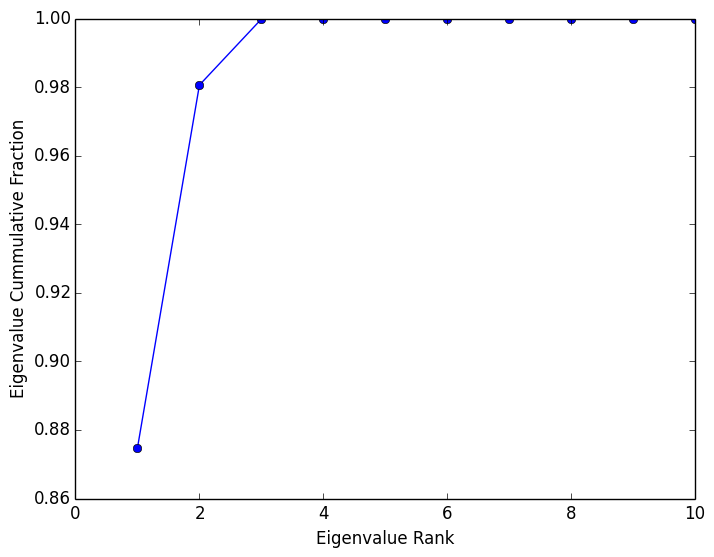
\includegraphics[scale=.75]{./Chapter4/pk_eigenvalues.png}
 \end{center}
\end{figure}
Note, each eigenvector consists of 500 time steps. From Fig. \ref{fig:pk_eigenvalues} it's clear that the three largest eigenvalues can explain over 99\% of the variance in the 100 samples. Consequently, the 500 dimensional space initially faced with in the point kinetics time series can be reduced to only three dimensions with minimal loss of explainability. 

The three principal components corresponding to the top three eigenvalues are plotted for training sizes of 20, 75, and 200 in Fig. \ref{fig:pk_eigenvectors} to ensure the shapes of the principal components do not change. It is important that the fundamental shapes of the principal components do not change significantly with training size because then surrogates for expansion coefficients values cannot be constructed since they are predicting different objects.   
\begin{figure}[!h]
\caption{\label{fig:pk_eigenvectors}
Top three principal components for the point kinetics time series as calculated using various training set sizes.}
 \begin{center}
  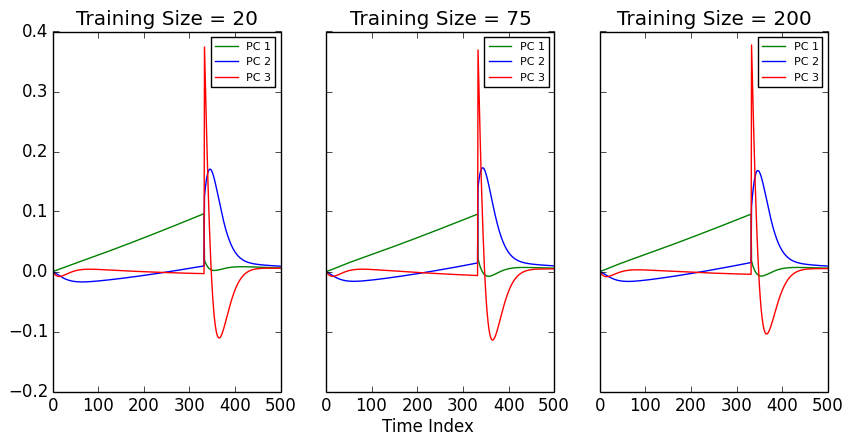
\includegraphics[scale=.7]{./Chapter4/pk_eigenvectors.png}
 \end{center}
\end{figure}
For deterministic computer codes, as those investigated in this thesis, the shapes of the principal components are expected to remain relatively static with training set size. Contrarily, the magnitudes of the principal components are expected to change as each principal component is expected to account for more variance introduced with increased training size. Indeed, such a phenomenon is observed in Fig. \ref{fig:pk_eigenvectors}. The first principal component in this problem closely follows the normalized reactor power while the second and third principal components correspond to the variance presented following the decrease in power once the sawtooth reactivity insertion ends.

To analyze how well the kriging surrogates are capable of predicting the principal component coefficients, the actual expansion coefficients are plotted against the predicted coefficients in Fig. \ref{fig:pk_45degree} for various training set sizes. The test set in this case consists of 50 \ac{LHS} sampled independently of those using the training sets. Note, the same test set is used for all proceeding analyses. As the training set size increases in Fig. \ref{fig:pk_45degree} the relationship between predicted and true expansion coefficients is gradually rotated to 45$^\circ$.      
\begin{figure}[!h]
\caption{\label{fig:pk_45degree}
Comparison of predicted and true principal component expansion coefficients for the point kinetics problem using 45$^\circ$ plots.}
 \begin{center}
  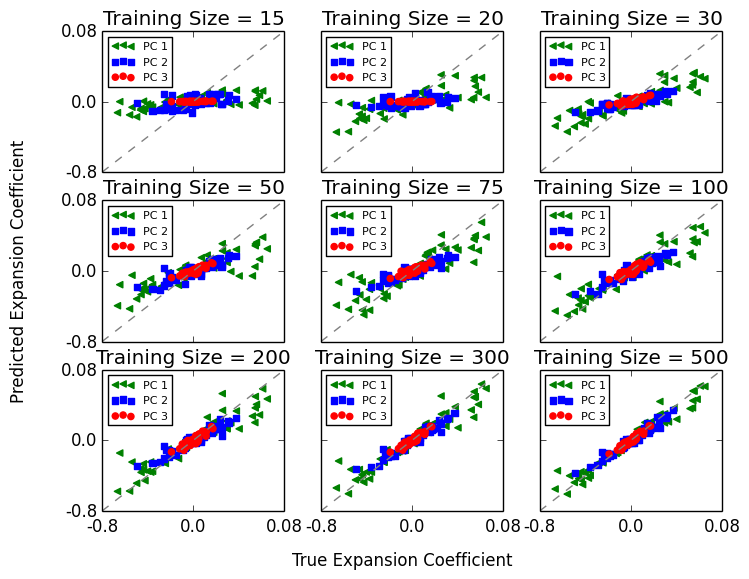
\includegraphics[scale=.7]{./Chapter4/pk_45degree.png}
 \end{center}
\end{figure}
For relatively low training sizes the predicted expansion coefficients are nearly zero, the mean value of the kriging surrogate. Part of the reason for this is the algorithm utilized for optimizing the $\theta$ values in the kriging construction. Although a global optimizer should be used a local optimization algorithm is generally used in R \cite{R} and Python statistical packages for efficiency. Regardless of the sample size in Fig. \ref{fig:pk_45degree} the surrogates struggle with predicting extreme expansion coefficients, which for this problem have magnitudes in the regions of -0.08 and 0.08. Since the expansion coefficients are normally distributed, as in Fig. \ref{fig:pk_coeff_distributions}, there simply are not as many training samples in these regions to provide accurate predictions. However, the kriging formulation is aware of this situation and accounts for the problem by outputting a relatively large uncertainty for these extreme expansion coefficients. 
\begin{figure}[!h]
\caption{\label{fig:pk_coeff_distributions}
Distributions of point kinetics principal component expansion coefficients for a training size of 500 samples.}
 \begin{center}
  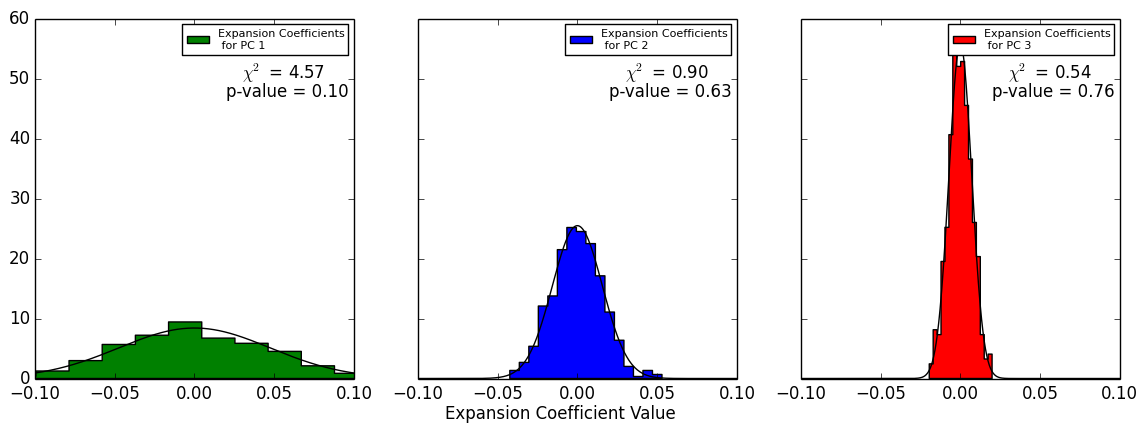
\includegraphics[scale=.5]{./Chapter4/pk_coeff_distributions.png}
 \end{center}
\end{figure} 

The performance of the time series kriging formulation, with uncertainties for the expansion coefficients accounted for, is gaged in Fig. \ref{fig:pk_stdzd_xval_residuals} by utilizing the standardized cross-validated residual in Eq. \ref{eq:stnd_xval_residual}.   
\begin{equation}
\label{eq:stnd_xval_residual}
 \frac{ p_{ij} - \hat{p}_{ij} }{ \sigma_{\hat{p}_{ij}} } . 
\end{equation}  
Since the expansion coefficients are normally distributed, some 99\% of the values' standardized values should lay between -3 and +3. From Fig. \ref{fig:pk_stdzd_xval_residuals} points lay outside the bounds only for the small train sizes consisting of 15 and 20 samples. Indeed, for small train set sizes the uncertainty predictions are likely to be misrepresented. Recall, kriging predictions are initialized by the mean of the objective function in the training set and then error terms are added based on the proximity of the desired inputs to those in the training set.  
\begin{figure}[!h]
\caption{\label{fig:pk_stdzd_xval_residuals}
Cross validation of the point kinetics time series surrogate by examining standardized cross-validated residuals.}
 \begin{center}
  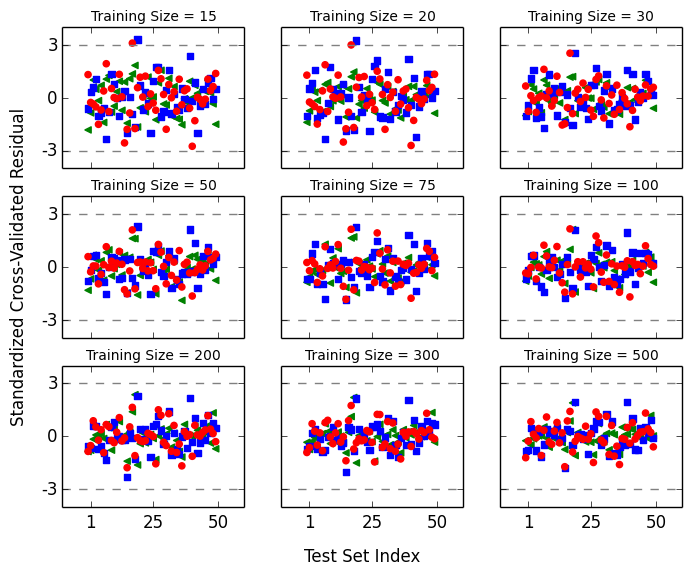
\includegraphics[scale=.7]{./Chapter4/pk_stdzd_xval_residuals.png}
 \end{center}
\end{figure} 
As expected, the standardized residuals decrease with increasing train set size. To visualize this trend better the absolute value of the standardized residuals are plotted against train set size in Fig. \ref{fig:pk_average_zscore}. After some 100 samples in the training set there appears to be only marginal gains in test set performance. Fig. \ref{fig:pk_average_zscore} indicates that the first principal component for the point kinetics time series surrogate is predicted best followed by the third and second principal components. Since each successive principal component captures less variance than its predecessors it is most important to accurately predict the principal components corresponding to the largest eigenvalues. 
\begin{figure}[!h]
\caption{\label{fig:pk_average_zscore}
Average absolute value of standardized cross-validated residuals for the point kinetics time series surrogate for various train set sizes.}
 \begin{center}
  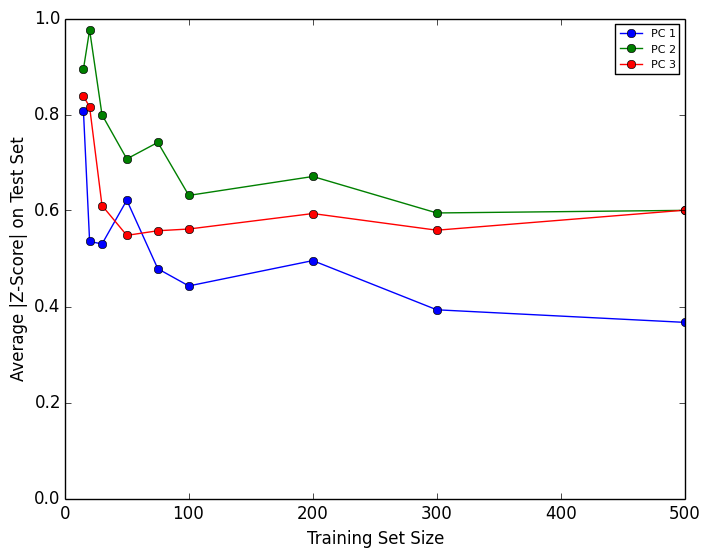
\includegraphics[scale=.7]{./Chapter4/pk_average_zscore.png}
 \end{center}
\end{figure}
 
  
